\chapter{短文本分类系统设计和实现}
本章主要阐述短文本分类系统的功能设计与代码实现,并详细介绍系统包含的各个功能模块。
整个系统可以分为离线网络训练与在线短文本分类两大部分,离线网络训练用于语料库更新以及
分类模型学习与参数调优,在线短文本分类则是系统实际提供的功能,用于给外部系统调用。
这两部分相互依赖,只有通过离线网络训练不断更新分类模型数据,
在网络训练时将模型参数调整到最优,才能让在线分类系统获得最好的效果。
\section{系统总体概述}
该短文本分类系统设计的主要目的是给其他用户提供一个持续可靠的短文本分类服务,主要思想是依据使用领域不断通过网络爬虫
搜集标注好的训练语料,训练出相应的词向量与字向量。然后系统使用这些文本表示信息训练分类
网络,并根据在验证集上的表现动态调节相关参数让模型效果达到最优。最后使用训练得到的网络参数
给前台用户提供短文本分类服务。系统的总体架构逻辑上大致可以分为三个子系统:
训练语料更新子系统、分类模型训练子系统和短文本分类子系统,整个流程如图\ref{system_architecture}所示。
\begin{figure}[h]
    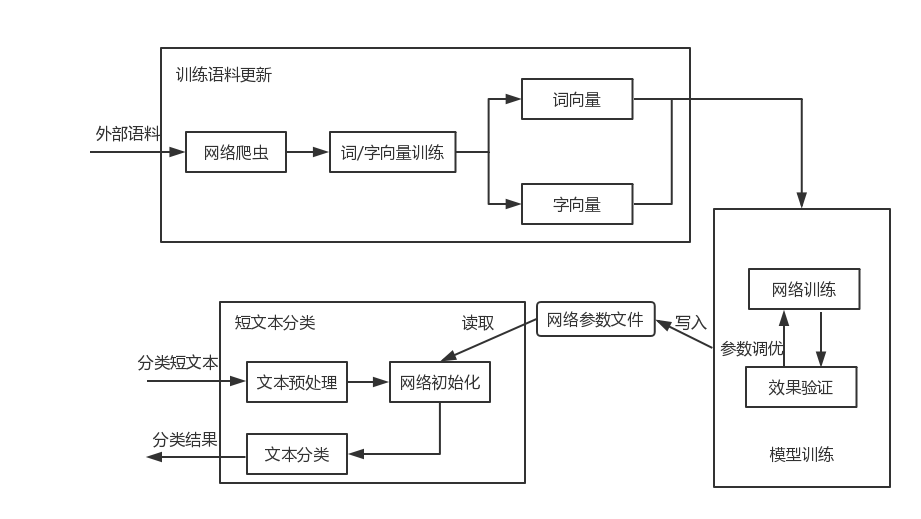
\includegraphics[scale=0.45]{picture/system_architecture.png}
    \caption{短文本分类系统流程}
    \label{system_architecture}
\end{figure}

为了保证系统的运算速度以及服务的稳定性,后台的语料更新子系统和短文本分类子系统都由包含多台
计算机的集群提供服务,分类模型训练子系统则为高性能运算服务器,配备有能够加速矩阵、向量计算
的NVIDIA Geforce显卡。系统的整体物理部署如图\ref{system_deployment}所示。
\begin{figure}[h]
    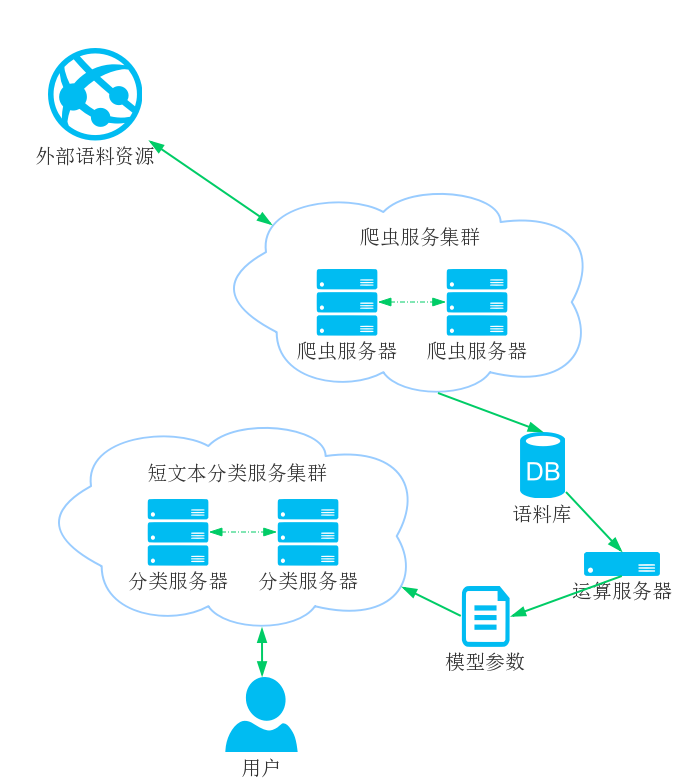
\includegraphics[scale=0.45]{picture/system_deployment.png}
    \caption{分类系统物理部署}
    \label{system_deployment}
\end{figure}
\section{系统各模块的设计和实现}
系统各个子系统的功能模块如图\ref{system_module}所示,训练语料更新子系统分为
网络爬虫、队列管理、语料数据存储、词/字向量训练四个模块,模型训练子系统分为
分类网络训练、参数调优两个模块,短文本分类子系统分为分类服务、日志记录两个模块。
其中训练语料更新子系统和模型训练子系统为后台模块,由系统定时启动,用于实时更新系统的
模型参数,短文本分类子系统为前台模块,用于与用户交互,给外部用户提供短文本分类服务。
下面对每一个功能模块进行详细阐述。
\begin{figure}[h]
    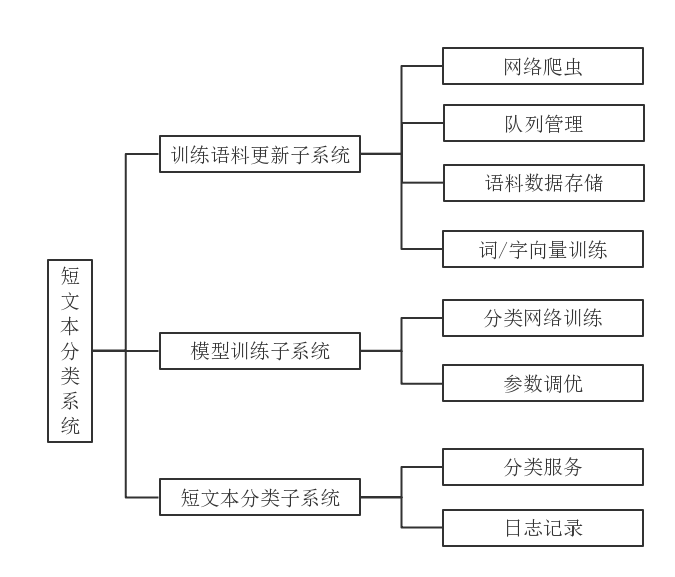
\includegraphics[scale=0.45]{picture/system_module.png}
    \caption{系统功能模块图}
    \label{system_module}
\end{figure}
\subsection{网络爬虫}
网络爬虫模块采用分布式爬虫架构,由多个网络节点中的爬虫程序共同完成数据抓取任务。
爬虫程序基于Python的Scrapy框架开发,
该框架是一个快速、
高层次的屏幕抓取和web抓取框架,用于抓取web站点并从页面中提取结构化的数据,
并且轻量灵活,能够快速的二次开发,适应不同爬虫需求。
\begin{figure}[h]
    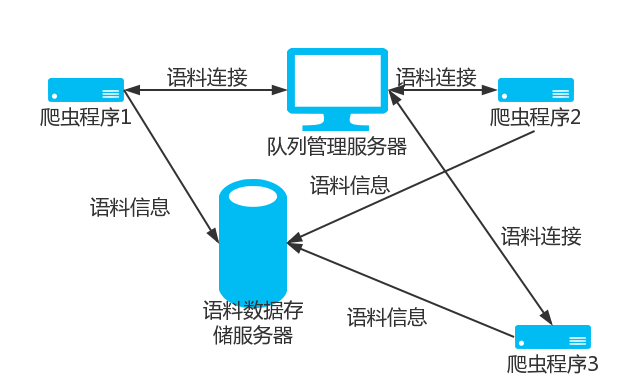
\includegraphics[scale=0.5]{picture/spider.png}
    \caption{网络爬虫模块结构图}
    \label{spider}
\end{figure}

爬虫模块的整体结构如图\ref{spider}所示,爬虫任务由队列管理模块分发,爬虫程序
负责数据的获取,然后将获取的数据写入语料数据存储模块。
每个爬虫程序包含4个组件:
\begin{itemize}
    \item[-] 下载器:负责通过http/https协议从外部WEB服务器下载WEB页面,以便后续的处理。
    \item[-] 页面解析器:负责解析下载的WEB页面,抽取所需的信息,以及发现新的语料链接并发送到队列管理模块。
    \item[-] 存储器:负责将获取的有用信息存储到语料数据存储模块。
    \item[-] IP池:负责给下载器提供代理IP,防止外部WEB服务器感知并禁止爬虫模块的请求。
\end{itemize}
\begin{figure}[!hbp]
    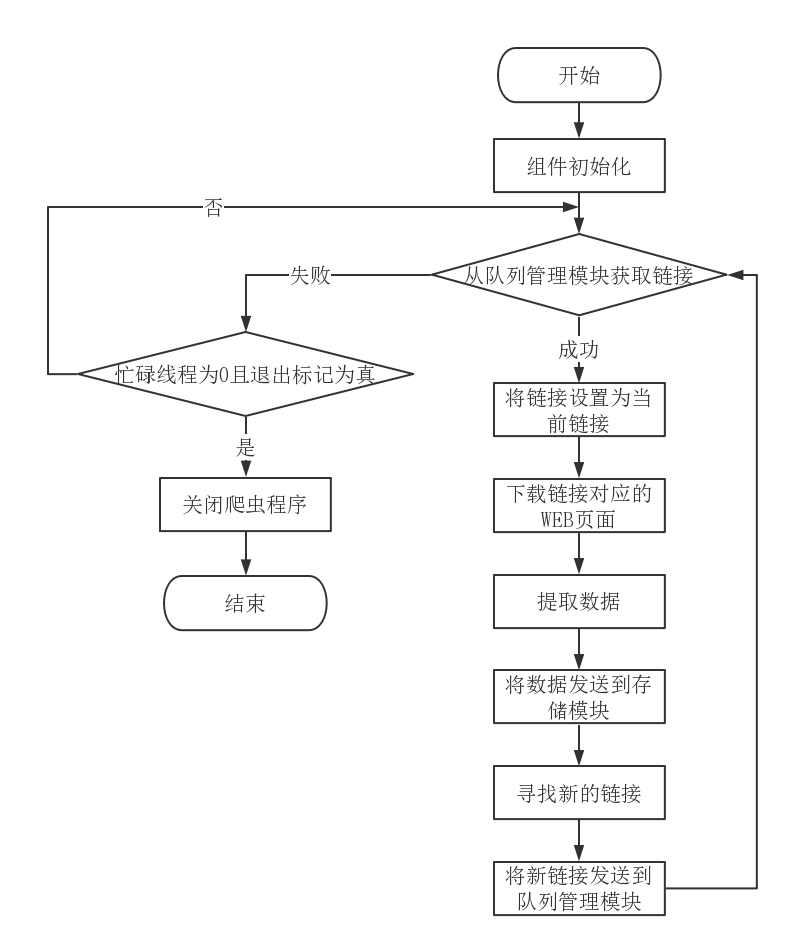
\includegraphics[scale=0.4]{picture/spider_flowchart.png}
    \caption{爬虫程序运行流程}
    \label{spider_flowchart}
\end{figure}

爬虫程序运行流程如图\ref{spider_flowchart}所示,首先,程序对各个组件进行初始化工作,
如生成下载器、设置线程池线程数量等。初始化结束之后,程序的主线程开始尝试从队列管理模块获取
下载链接,如果获取成功,则生成一个Task任务块并将其设置为当前任务,然后从线程池中取出一个线程进行下一步的处理,
如果获取失败,则认为当前任务可能已经结束,并检测退出标志是否为真以及是否还有工作中的线程,
两者都为真时表示系统已经确定退出,程序会立即关闭线程池,结束工作。
子线程接收到Task任务块会立刻运行下载器下载对应的WEB页面,下载完成后则通过页面解析器进行解析,然后
将解析得到的所需数据以及新的连接分别发送到语料信息存储模块和队列管理模块。
爬虫程序的核心页面处理代码如下所示:
\begin{lstlisting}[language={Python},frame=shadowbox,rulesepcolor=\color{red!0!green!0!blue!0}] 
    def parse(self, response):
    news = json.loads(response.body.decode('utf-8'))
    if news["message"] == "error":
        # 服务器返回错误数据,当前IP地址可能被禁止
        if "proxy" in response.meta:
            self.ban_ip[response.meta["proxy"]] = 1
        else:
            self.ban_ip[""] = 1
        print("ban ip: " + str(len(self.ban_ip)) + "/" + str(len(IP_POOL)))
        if len(self.ban_ip) >= len(IP_POOL):
            raise CloseSpider("ban")
        yield Request(response.url, dont_filter=True)
    else:
        # 获取新闻语料
        news_list = news["data"]
        for news_item in news_list:
            item = NewsSpiderItem()
            if "chinese_tag" not in news_item or news_item["chinese_tag"] == "其他" or \
               news_item["chinese_tag"] == "视频":
                continue
            item["tag"] = news_item["chinese_tag"]
            item["title"] = news_item["title"]
            item["hash"] = self.__get_md5(news_item["title"].encode("utf-8"))
            # 返回获取的数据
            yield item
        next_time = news["next"]["max_behot_time"]
        sign = lib.get_sign(next_time)
        ascp_dict = lib.get_as_cp()
\end{lstlisting}
\begin{lstlisting}[language={Python},frame=shadowbox,rulesepcolor=\color{red!0!green!0!blue!0}] 
        # 返回新发现的链接
        yield Request(self.api_format % (self.__get_url_tag(response.url), next_time, next_time,
                                         ascp_dict["as"], ascp_dict['cp'], sign))
\end{lstlisting}
\subsection{队列管理}
队列管理模块主要用来给整个爬虫网络提供一个可靠的任务管理服务,统一分发数据爬取任务,
平衡各节点的工作负担,负载均衡,防止忙碌节点的出现。模块以稳定性、实时性较好的
Redis(REmote DIctionary Server)分布式数据库为基础实现,通过将爬虫程序
上传的新链接重新分配给网络中的其他节点,不断推进整体的数据爬取进度,工作示意图大致
如图\ref{redis}所示。
\begin{figure}[h]
    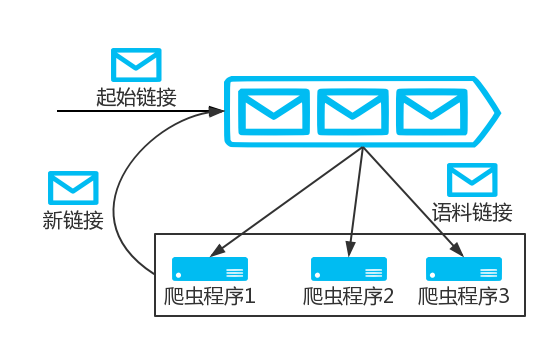
\includegraphics[scale=0.5]{picture/redis.png}
    \caption{队列管理模块工作示意图}
    \label{redis}
\end{figure}
\subsection{语料数据存储}
语料数据存储模块用于持久化保存爬虫程序提取的语料信息,使用Mysql数据库实现。
为了获取语料的全面信息,语料数据存储模块除了存储语料文本,还存储了来源、URL链接、
发布时间、爬取时间、文本MD5等重要信息,以新闻标题语料为例,相关数据格式如表\ref{news_struct_table}所示,
爬取的相应数据见表\ref{news_data_table}所示。

\begin{table}[h]
    \caption{新闻标题语料数据格式}
    \begin{tabular}{|c|c|c|c|}
        \hline
        title & 新闻的标题 & url & 新闻的url地址 \\
        \hline
        time & 新闻的发布时间 & get\_time & 新闻的爬取时间 \\
        \hline
        resource & 新闻的来源 & news\_id & 新闻的id \\
        \hline
        news\_md5 & 新闻标题文本的md5值 & category & 新闻所属的类别  \\
        \hline
    \end{tabular}
    \label{news_struct_table}
    \end{table}

\begin{table}[h]
    \caption{爬取的新闻标题数据}
    \begin{tabular}{|c|c|}
        \hline
        title & 男子出狱创业招500名犯人,为帮员工戒毒半年吃素 \\
        \hline
        url & http://toutiao.com/group/6504029172468285966/ \\
        \hline
        time & 1511756299 \\
        \hline
        get\_time & 1511759149 \\
        \hline
         category & 社会 \\
        \hline
        resource & 人民网 \\
        \hline
        news\_id & 6504029172468285966 \\
        \hline
        news\_md5 &  1ce5761e192c42e76e4bb45ac22be5ed \\
        \hline
    \end{tabular}
    \label{news_data_table}
    \end{table}

同时,为了后续模块能够方便的处理爬取的语料数据,存储模块还需要对这些数据进行预处理工作,
包括标点符号剔除、分词处理、繁简转换、分词筛选、去除停用词、汉字统计。
其中标点符号剔除、分词处理、繁简转换和之前小节介绍的一样,这里不再赘述,分词筛选是用于统计
语料中发现的新词,汉字统计则是统计新汉字,这两者是判断是否需要更新词向量/字向量的重要指标。去除停用词使用的是
哈工大、百度、川大的停用词列表,能够有效去除语料中对语义特征没有帮助的词。同样以新闻标题数据为例,
预处理之后的数据如表\ref{pretreatment_data_table}所示。
\begin{table}[h]
    \caption{预处理过后的新闻数据}
    \begin{tabular}{|c|c|}
        \hline
        id & 1303086993 \\
        \hline
        news\_id & 6504029172468285966 \\
        \hline
        words & 男子,出獄,創業,招,犯人,幫,員工,戒毒,半,年,吃,素 \\
        \hline
        char & 男,子,出,獄,創,業,招,犯,人,幫,員,工,戒,毒,半,年,吃,素 \\
        \hline
    \end{tabular}
    \label{pretreatment_data_table}
    \end{table}
\subsection{字/词向量训练}
字/词向量训练模块主要用来获取分类模型使用的词向量与字向量,采用增量训练的方式,
只有在语料数据或新词/新字数量超过一定阈值的时候,才开始训练,更新当前使用的词/字向量。

由\ref{recwe_section}节的目标公式以及负采样算法可以继续推导得式\ref{neg_eqn}:
\begin{equation}
    \begin{aligned}
        L &= \sum_{w\in l}\sum_{u\in \left \{ w \right \}\cup NEG\left ( w \right )}\left \{ L^w\left ( u \right ) \cdot \log \left [ \sigma \left ( X_w^{\top }\theta^u  \right ) \right ]+\left [ 1-  L^w\left ( u \right )\right ]\cdot \log \left [1- \sigma \left ( X_w^{\top }\theta^u  \right ) \right ]\right \} \\
        &+ \sum_{c\in l}\sum_{u\in \left \{ c \right \}\cup NEG\left ( c \right )}\left \{ L^c\left ( u \right ) \cdot \log \left [ \sigma \left ( X_c^{\top }\theta^u  \right ) \right ]+\left [ 1-  L^c\left ( u \right )\right ]\cdot \log \left [1- \sigma \left ( X_c^{\top }\theta^u  \right ) \right ]\right \}
    \end{aligned}
    \label{neg_eqn}
\end{equation}

再根据式\ref{neg_eqn}分别对各个参数求导,即可得到词向量/字向量的梯度更新方法,如公式所示\ref{neg_update_eqn}。
\begin{equation}
    \begin{aligned}
        q&=\sigma \left ( X_w^\top \theta^u \right )\\
        g&=\eta \left ( L^w\left ( u \right )-q \right )\\
        e &:=e+g\theta^u\\
        \theta^u &:=\theta^u+gX_w\\
        v_u &:=v_u+e
    \end{aligned}
    \label{neg_update_eqn}
\end{equation}

词/向量训练代码由C语言实现,核心部分分为正向推导、梯度计算、反向更新三个部分。
正向推导主要是从模型底部统计所有输入向量,得到当前预测的隐藏层向量,对应的代码如下所示:
\begin{lstlisting}[language={[ANSI]C},frame=shadowbox,rulesepcolor=\color{red!0!green!0!blue!0}] 
    //叠加窗口内的词向量
    for(c = 0; c < layer1_size; c++) 
        neu1[c] += syn0[c + last_word * layer1_size];
    //叠加字向量
    for(c = 0; c < vocab[last_word].character_size; c++)
    {
        char_id = vocab[last_word].character[c];
        char_id_list[char_list_cnt++] = char_id;
        for(d = 0; d < layer1_size; d++) neucomp[d] += synchar[d + char_id * layer1_size];
        for(d = 0; d < char2comp[char_id].comp_size; d++)
        {
            comp_id = char2comp[char_id].comp[d];
            if(comp_id != char_id)
            {
                comp_id_list[comp_list_cnt++] = comp_id;
                //叠加部首向量
                for(e = 0; e < layer1_size; e++) neucomp[e] += synchar[e + comp_id * layer1_size];
            }
        }
    }
\end{lstlisting}

梯度计算部分是根据公式\label{neg_update_eqn}计算当前输入对应的梯度,代码如下所示。
\begin{lstlisting}[language={[ANSI]C},frame=shadowbox,rulesepcolor=\color{red!0!green!0!blue!0}] 
    
for(d = 0; d < negative + 1; d++)
{
    //一些初始化操作
    ...
    // 开始计算梯度
    l2 = target * layer1_size;
    real f1 = 0, f3 = 0, g1 = 0, g3 = 0;
    for(c = 0; c < layer1_size; c++)
    {
        f1 += neu1[c] * syn1neg[c + l2];
        f3 += neucomp[c] * syn1neg[c + l2];
    }
    //f1
    if(f1 > MAX_EXP)
        g1 = (label - 1) * alpha;
    else if(f1 < -MAX_EXP)
        g1 = (label - 0) * alpha;
    else
        g1 = (label - expTable[(int) ((f1 + MAX_EXP) * (EXP_TABLE_SIZE / MAX_EXP / 2))]) * alpha;

    //f3
    if(f3 > MAX_EXP)
        g3 = (label - 1) * alpha;
    else if(f3 < -MAX_EXP)
        g3 = (label - 0) * alpha;
    else
        g3 = (label - expTable[(int) ((f3 + MAX_EXP) * (EXP_TABLE_SIZE / MAX_EXP / 2))]) * alpha;
    // 统计梯度
    for(c = 0; c < layer1_size; c++)
    {
        neu1_grad[c] += g1 * syn1neg[c + l2];
        neucomp_grad[c] += g3 * syn1neg[c + l2];
    }
    //更新 syn1neg
    for(c = 0; c < layer1_size; c++)
        syn1neg[c + l2] += g1 * neu1[c] + g3 * neucomp[c];
    
}
\end{lstlisting}

反向更新部分则是用上个部分得到的梯度更新输入的词向量与字向量及部首向量,完成一次训练,相关代码如下所示:
\begin{lstlisting}[language={[ANSI]C},frame=shadowbox,rulesepcolor=\color{red!0!green!0!blue!0}] 
for(a = b; a < window * 2 + 1 - b; a++)
    if(a != window)
    {
        c = sentence_position - window + a;
        if(c < 0) continue;
        if(c >= sentence_length) continue;
        last_word = sen[c];
        if(last_word == -1) continue;
        for(c = 0; c < layer1_size; c++)
        {
            //更新词向量
            syn0[c + last_word * layer1_size] += neu1_grad[c] / cw;
        }
    }
    for(a = 0; a < char_list_cnt; a++)
    {
        char_id = char_id_list[a];
        for(c = 0; c < layer1_size; c++)
        {
            //更新字向量
            synchar[c + char_id * layer1_size] += neucomp_grad[c] / (char_list_cnt + comp_list_cnt);
        }
    }
    for(a = 0; a < comp_list_cnt; a++)
    {
        comp_id = comp_id_list[a];
        for(c = 0; c < layer1_size; c++)
        {
            //更新部首向量
            synchar[c + comp_id * layer1_size] += neucomp_grad[c] / (char_list_cnt + comp_list_cnt);
        }
    }
\end{lstlisting}
\subsection{模型训练}
模型训练子系统包含分类网络训练与参数调优两个模块,是整个系统的核心部分,用于训练并获取
分类性能最优的网络模型参数。详细过程设计如图\ref{train}所示。
\begin{figure}[!hbp]
    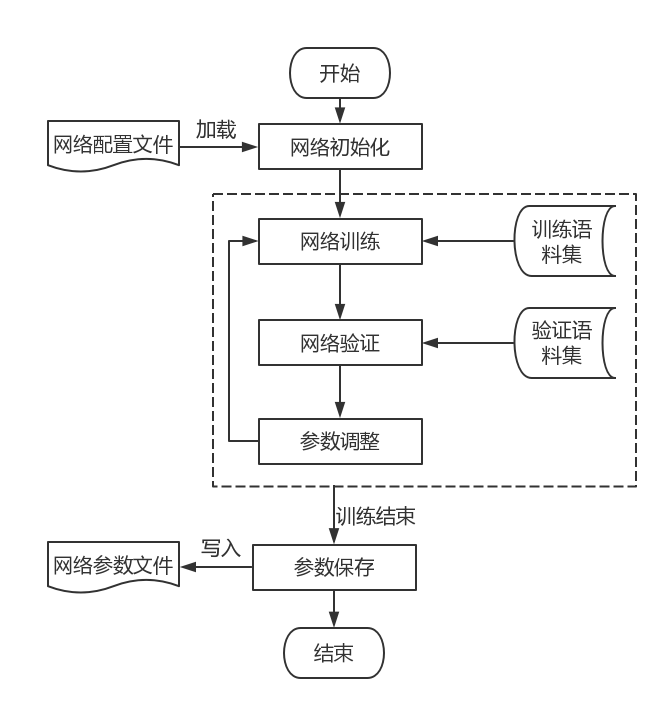
\includegraphics[scale=0.6]{picture/train.png}
    \caption{模型训练子系统过程示意图}
    \label{train}
\end{figure}

模型训练子系统的详细流程如下:
\begin{enumerate}
    \item 根据配置文件中的相关配置信息使用Google Tensorflow深度学习框架构建
    \ref{4_section}中提出的短文本分类网络结构。
    \item 使用误差反向传播算法(Error Back Propagation,BP)不断进行前向计算与后向
    传导,更新网络参数。
    \item 使用验证语料集对训练好的网络进行测试,确定网络的性能以及判断网络是否正确
    收敛。验证语料集不参与网络训练,仅仅在其上进行BP算法的前向过程。
    \item 根据相关配置文件,在一定范围内微调网络的参数并使用新参数重新训练玩了个,
    尝试优化网络。在调整一定次数之后,取性能最好的网络参数作为最后的有效参数。
    \item 保存完成调优之后的网络参数,以便后续阶段使用。
    \end{enumerate}

表\ref{net_data_alert_table}展示了需要调节的网络参数及其调节范围,参数微调时会在范围内对相关参数重新取值。
图\ref{train_tmp_data}展示了系统保存的网络参数,训练过程中产生所有模型参数都会被保存并统一编号,方便日后管理
人员分析。
\begin{table}[h]
    \caption{微调参数列表}
    \begin{tabular}{|c|c|}
        \hline
        参数名称 & 调节范围 \\
        \hline
         LSTM隐藏层大小 & 64-256 \\
        \hline
        CNN卷积核数量 & 64-256 \\
        \hline
        CNN卷积核高度 & 2-10 \\
        \hline
        Dropout层丢弃率 & 0.2-0.6 \\
        \hline
        学习率 & 0.001-0.0001 \\
        \hline
        Attention层大小 & 65-256 \\
        \hline
    \end{tabular}
    \label{net_data_alert_table}
    \end{table}

\begin{figure}[!hbp]
    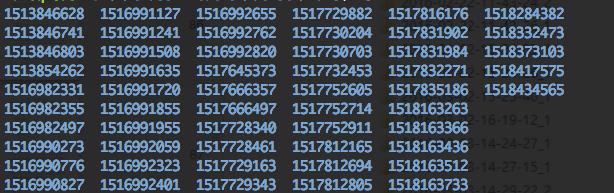
\includegraphics[scale=0.6]{picture/train_tmp_data.png}
    \caption{模型保存的网络参数文件}
    \label{train_tmp_data}
\end{figure}
\subsection{分类服务}
分类服务模块主要是给外部用户提供一个持续有效的即时短文本分类服务,
整个服务依托于HTTP协议,通过传递Json进行数据交换,外部用户只要按照格式要求
给系统发送JSON数据,系统即会返回分类结果。服务网络由多台服务节点组成,并使用
Nginx反向代理服务器提供链接分发服务,保证系统的稳定性以及可拓展性,具体框架如图\ref{server_chart}所示。
\begin{figure}[!hbp]
    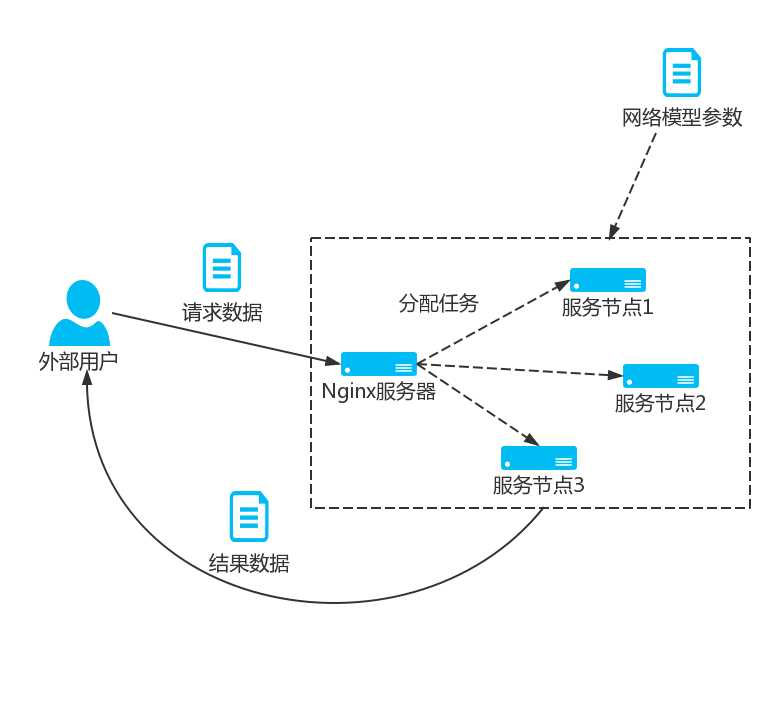
\includegraphics[scale=0.6]{picture/server_chart.png}
    \caption{分类服务模块基本框架示意图}
    \label{server_chart}
\end{figure}

用户的分类请求首先发往Nginx代理服务器,由代理服务器统一分配服务节点。服务节点接收到分类文本之后,
需要对其分词、去除标点与停用词,然后按照词/字向量表转换为对应的词向量/字向量数据,同时忽略词表/字表中没有词或字。
最后将数据送入分类网络,并将分类结果返回给用户。
\subsection{日志记录}
日志记录模块用于记录外部用户的相关信息,记录内容包括用户编号、用户IP、分类文本等,
同时系统的分类结果也会被保存,方便以后的查阅以及错误排查。日志存储模块使用Mongodb
作为存储数据库。Mongodb与常见的Mysql数据库等关系数据库不同,采用非关系结构存储数据,
同时侧重大量数据写入性能,非常适合日志信息存储。用户日志的具体信息如表\ref{log_table}所示。
\begin{table}[h]
    \caption{用户日志字段}
    \begin{tabular}{|c|c|}
        \hline
        字段名称 & 字段值 \\
        \hline
        \_id & ObjectId("41d2c2913761a2258c7c4e79") \\
        \hline
        user\_id & dca8815bef5e1150 \\
        \hline
        time & 2016-01-27 05:55 \\
        \hline
        model\_arg & 1517812805 \\
        \hline
        content & 如果一个人临去世之前把信用卡全部套现,银行会怎么办? \\
        \hline
        classification\_result & 财经 \\
        \hline
    \end{tabular}
    \label{log_table}
    \end{table}

\section{系统测试与分析}
为了验证系统的有效性以及在最新短文本语料数据上的分类效果,
需要在实际网络环境中进行系统测试,并对系统的测试结果进行统计、分析。
本文将在今日头条新闻网站的标题数据上对系统进行实际的测试。
\subsection{新闻标题数据搜索}
\subsection{汉字信息库}
\subsection{分类测试结果}
\section{本章小节}